\begin{frame}{Reaction}

  \vspace{-0.16cm}

  \begin{columns}[c,onlytextwidth]

    \begin{column}{0.58\textwidth}
      {\color{HydraMuted}\fontsize{8.2}{10.2}\selectfont
        Begin with a system of ordinary differential equations
      \par}

      \vspace{-0.22cm}

      {\color{HydraWhite}\fontsize{10.4}{13.2}\selectfont
      \begin{align*}
        \partial_t u&=f(u,v)
        \\
        \partial_t v&=g(u,v)
      \end{align*}
      }

      \vspace{-0.28cm}

      {\color{HydraWhite}\fontsize{8.2}{10.2}\selectfont
        $u$ and $v$ are the local concentrations of two substances
      \par}

      \vspace{0.10cm}

      {\color{HydraMuted}\fontsize{8.2}{10.2}\selectfont
        The functions $f(u,v)$ and $g(u,v)$ describe how these
        concentrations change depending on their current values
      \par}

      \vspace{0.24cm}

      \HydraPoint[HydraGold]
        {One state at every position}
        {The pair $(u,v)$ represents the local chemical state.}

      \vspace{-0.28cm}

    \end{column}

    \begin{column}{0.38\textwidth}
      \centering

      % REPLACEABLE VISUAL
      % Replace the tikzpicture with:
      % \includegraphics[width=\linewidth,height=5.25cm,keepaspectratio]{figures/local_dynamics/...}
      \begin{tikzpicture}[x=0.86cm,y=0.82cm]

        \draw[-{Latex[length=2mm]},HydraMuted,line width=0.75pt]
          (0.45,0.55) -- (5.25,0.55)
          node[below,text=HydraMuted,
            font=\fontsize{7}{8.2}\selectfont] {$u$};

        \draw[-{Latex[length=2mm]},HydraMuted,line width=0.75pt]
          (0.55,0.45) -- (0.55,5.25)
          node[left,text=HydraMuted,
            font=\fontsize{7}{8.2}\selectfont] {$v$};

        \fill[HydraGold]
          (1.15,3.10) circle[radius=0.085cm];

        \fill[HydraCyan]
          (2.70,1.55) circle[radius=0.085cm];

        \fill[HydraViolet]
          (4.20,3.85) circle[radius=0.085cm];

        \draw[-{Latex[length=2.1mm]},HydraGold,line width=1.2pt]
          (1.15,3.10) -- ++(0.62,0.32);

        \draw[-{Latex[length=2.1mm]},HydraCyan,line width=1.2pt]
          (2.70,1.55) -- ++(0.45,0.70);

        \draw[-{Latex[length=2.1mm]},HydraViolet,line width=1.2pt]
          (4.20,3.85) -- ++(-0.70,-0.24);

        \node[anchor=north,text=HydraMuted,
          text width=4.7cm,align=center,
          font=\fontsize{7.2}{8.8}\selectfont]
          at (2.85,0.05)
          {the vector $(f(u,v),g(u,v))$ determines the direction of change};

      \end{tikzpicture}
    \end{column}

  \end{columns}

\end{frame}


\begin{frame}{Reaction --- vector field and trajectory}

  \vspace{-0.04cm}

  \begin{columns}[c,onlytextwidth]

    \begin{column}{0.43\textwidth}
      {\color{HydraWhite}\fontsize{11.6}{14.6}\selectfont
      \[
        \begin{aligned}
          \partial_t u&=f(u,v)
          \\
          \partial_t v&=g(u,v)
        \end{aligned}
      \]
      }

      \vspace{-0.14cm}

      {\color{HydraMuted}\fontsize{8.2}{10.2}\selectfont
        supplemented with initial conditions
      \par}

      \vspace{-0.22cm}

      {\color{HydraWhite}\fontsize{10.2}{13}\selectfont
      \[
        u_0=u(0)
        \qquad
        v_0=v(0)
      \]
      }

      \vspace{-0.24cm}

      \HydraPoint[HydraGold]
        {Initial state}
        {The pair $(u_0,v_0)$ selects the starting point in the concentration plane.}

      \vspace{-0.10cm}

      \HydraPoint[HydraCyan]
        {Velocity}
        {The vector $(f(u,v),g(u,v))$ gives the instantaneous direction of change.}

      \vspace{-0.10cm}

      \HydraPoint[HydraGold]
        {Trajectory}
        {The solution curve is tangent to the vector field at every point.}
    \end{column}

    \begin{column}{0.53\textwidth}
      
      % \vspace{3.58cm}
      \centering

      % REPLACEABLE VISUAL
      % Replace the placeholder with:
      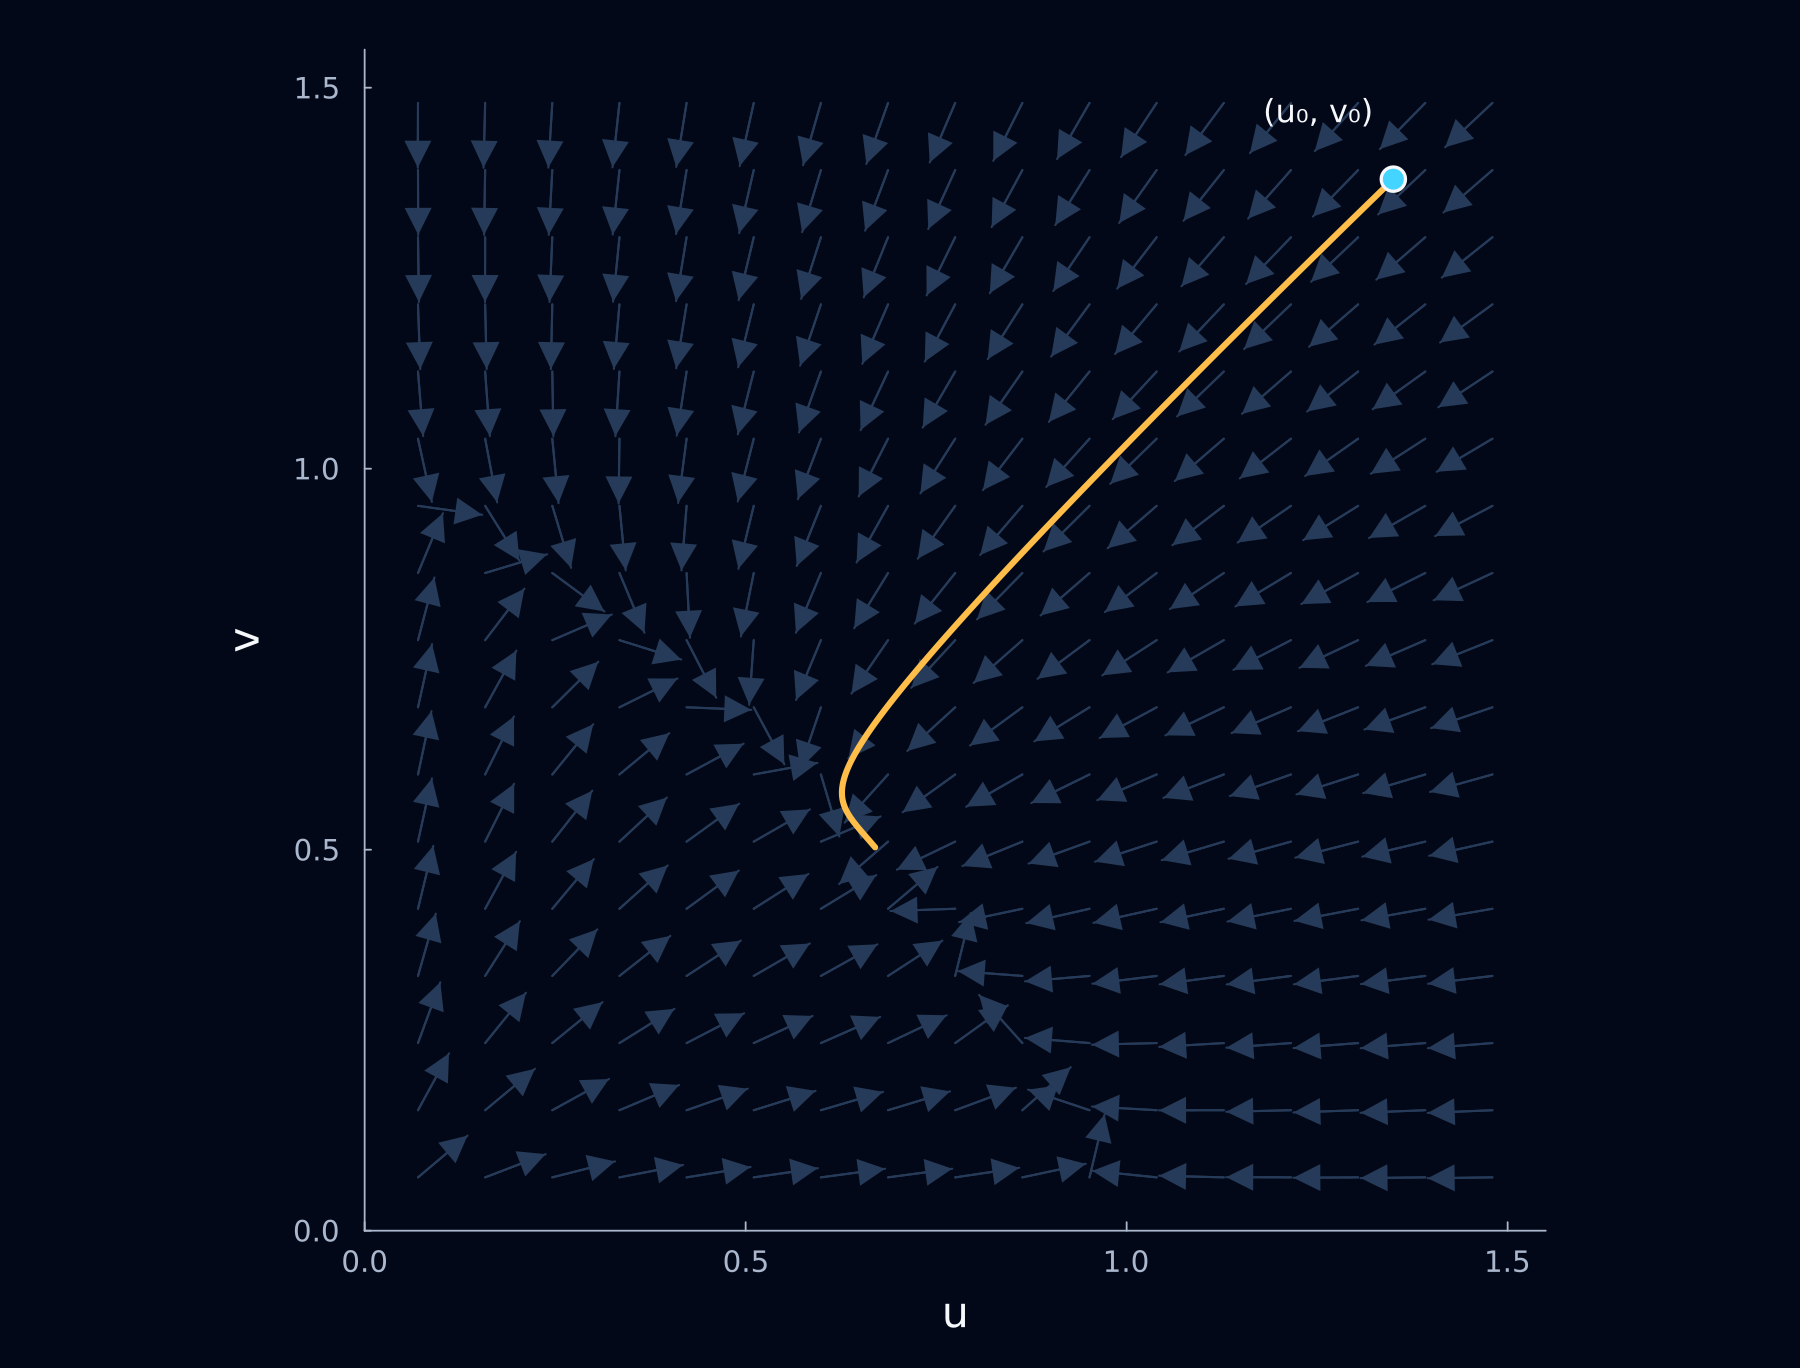
\includegraphics[
        width=\linewidth,
        height=5.45cm,
        keepaspectratio
      ]{figures/local_dynamics/vector_field.png}

      % \begin{tikzpicture}
      %   \node[
      %     draw=HydraLine,
      %     rounded corners=2pt,
      %     minimum width=0.94\linewidth,
      %     minimum height=5.25cm,
      %     align=center,
      %     text=HydraMuted,
      %     font=\fontsize{8}{10}\selectfont
      %   ] {
      %     vector field and trajectory
      %     \\
      %     \vspace{0.08cm}
      %     {\fontsize{6.8}{8.2}\selectfont
      %       replace with your own plot}
      %   };
      % \end{tikzpicture}
    \end{column}

  \end{columns}

\end{frame}

\begin{frame}{Steady state}

  \vspace{-0.12cm}

  \begin{columns}[c,onlytextwidth]


    
    \begin{column}{0.46\textwidth}
            {\color{HydraMuted}\fontsize{8.1}{10.2}\selectfont
        At a steady state $u(t)\equiv\bar u$, $v(t)\equiv\bar v$, both concentrations remain constant in time
      \par}


      {\color{HydraWhite}\fontsize{11.2}{14.2}\selectfont
      \[
        \begin{aligned}
          f(\bar u,\bar v)&=0
          &\qquad
          g(\bar u,\bar v)&=0
        \end{aligned}
      \]
      }

      \vspace{-0.22cm}


      \vspace{0.34cm}

      {\color{HydraWhite}\bfseries\fontsize{8}{9.6}\selectfont
        NULLCLINES\par}

      \vspace{-0.10cm}

      {\color{HydraWhite}\fontsize{11}{14}\selectfont
      \begin{align*}
        \textcolor{HydraCyan}{f(u,v)=0}
        &&
        \text{\color{HydraMuted}\fontsize{7.6}{9}\selectfont
          $u$ does not change}
        \\
        \textcolor{HydraGold}{g(u,v)=0}
        &&
        \text{\color{HydraMuted}\fontsize{7.6}{9}\selectfont
          $v$ does not change}
      \end{align*}
      }

      \vspace{-0.12cm}

      {\color{HydraMuted}\fontsize{8.1}{10.2}\selectfont
        Each nullcline contains states for which one concentration
        is instantaneously stationary
      \par}


    \end{column}

    \begin{column}{0.50\textwidth}
      \centering

      % REPLACEABLE VISUAL
      % Replace the tikzpicture with:
      % \includegraphics[
      %   width=\linewidth,
      %   height=5.40cm,
      %   keepaspectratio
      % ]{figures/local_dynamics/nullclines.png}

      \begin{tikzpicture}[x=0.88cm,y=0.82cm]
        \draw[-{Latex[length=2.3mm]},HydraMuted,line width=0.75pt]
          (0.40,0.48) -- (6.75,0.48)
          node[below,text=HydraMuted,
            font=\fontsize{7}{8.2}\selectfont] {$u$};

        \draw[-{Latex[length=2.3mm]},HydraMuted,line width=0.75pt]
          (0.50,0.38) -- (0.50,5.55)
          node[left,text=HydraMuted,
            font=\fontsize{7}{8.2}\selectfont] {$v$};

        \draw[
          HydraCyan,
          line width=1.65pt,
          domain=0.45:5.95,
          samples=90
        ]
          plot (\x,{0.60+0.12*\x*\x});

        \draw[HydraGold,line width=1.65pt]
          (0.55,4.00) -- (5.95,1.03);

        \node[
          anchor=west,
          text=HydraCyan,
          font=\bfseries\fontsize{8}{9.5}\selectfont
        ]
          at (3.95,4.70) {$f(u,v)=0$};

        \node[
          anchor=west,
          text=HydraGold,
          font=\bfseries\fontsize{8}{9.5}\selectfont
        ]
          at (5.65,1.35) {$g(u,v)=0$};

        \fill[HydraWhite]
          (3.72,2.26) circle[radius=0.10cm];

        \draw[HydraWhite,line width=0.75pt]
          (3.72,2.26) circle[radius=0.18cm];

        \node[
          anchor=south west,
          text=HydraWhite,
          font=\bfseries\fontsize{8}{9.5}\selectfont
        ]
          at (4.22,2.23)
          {steady state $(\bar u,\bar v)$};

        \draw[dashed,HydraLine,line width=0.65pt]
          (3.72,0.48) -- (3.72,2.26);

        \draw[dashed,HydraLine,line width=0.65pt]
          (0.50,2.26) -- (3.72,2.26);

        \node[
          anchor=north,
          text=HydraMuted,
          font=\fontsize{7.2}{8.8}\selectfont
        ]
          at (3.72,0.38) {$\bar u$};

        \node[
          anchor=east,
          text=HydraMuted,
          font=\fontsize{7.2}{8.8}\selectfont
        ]
          at (0.42,2.26) {$\bar v$};

        \node[
          anchor=north,
          text=HydraMuted,
          text width=5.6cm,
          align=center,
          font=\fontsize{7.2}{8.8}\selectfont
        ]
          at (3.55,-0.12)
          {the nullclines organize the local phase plane};
      \end{tikzpicture}
    \end{column}

  \end{columns}

\end{frame}


\begin{frame}{Lyapunov stability}

  \vspace{-0.54cm}

  \begin{columns}[c,onlytextwidth]

    \begin{column}{0.44\textwidth}
      {\color{HydraMuted}\fontsize{7.8}{9.6}\selectfont
        Consider two solutions of the same system
      \par}

      \vspace{-0.18cm}

      {\color{HydraWhite}\fontsize{9.7}{12.4}\selectfont
      \begin{align*}
        \partial_t u&=f(u,v)
        \\
        \partial_t v&=g(u,v)
      \end{align*}
      }

      \vspace{-1.28cm}

      {\fontsize{8.8}{11.2}\selectfont
      \begin{align*}
        \textcolor{HydraCyan}{u(0)}
        &\textcolor{HydraCyan}{=u_0}
        &
        \textcolor{HydraGold}{\widetilde u(0)}
        &\textcolor{HydraGold}{=\widetilde u_0}
        \\
        \textcolor{HydraCyan}{v(0)}
        &\textcolor{HydraCyan}{=v_0}
        &
        \textcolor{HydraGold}{\widetilde v(0)}
        &\textcolor{HydraGold}{=\widetilde v_0}
      \end{align*}
      }
      \par
      \vspace{0.1cm}

      {\color{HydraGold}\bfseries\fontsize{7.7}{9.2}\selectfont
        LYAPUNOV STABILITY\par}

      % \vspace{-0.10cm}

      {\color{HydraWhite}\fontsize{7.5}{9.3}\selectfont
        For every $\varepsilon>0$ there exists $\delta>0$ such that
      \par}

      \vspace{-0.42cm}

{\color{HydraWhite}\fontsize{9.4}{12}\selectfont
\begin{align*}
  \left\|
    (u_0,v_0)-(\widetilde u_0,\widetilde v_0)
  \right\|&<\delta
  \quad \Rightarrow  \\ 
  \left\|
    (u(t),v(t))-(\widetilde u(t),\widetilde v(t))
  \right\|&<\varepsilon
  \qquad
  \text{for all } t\geq0
\end{align*}
}
      \par
      \vspace{-0.26cm}

    \end{column}

    \begin{column}{0.52\textwidth}

        \begin{columns}[c,onlytextwidth]

          \begin{column}{0.72\linewidth}
            \centering

            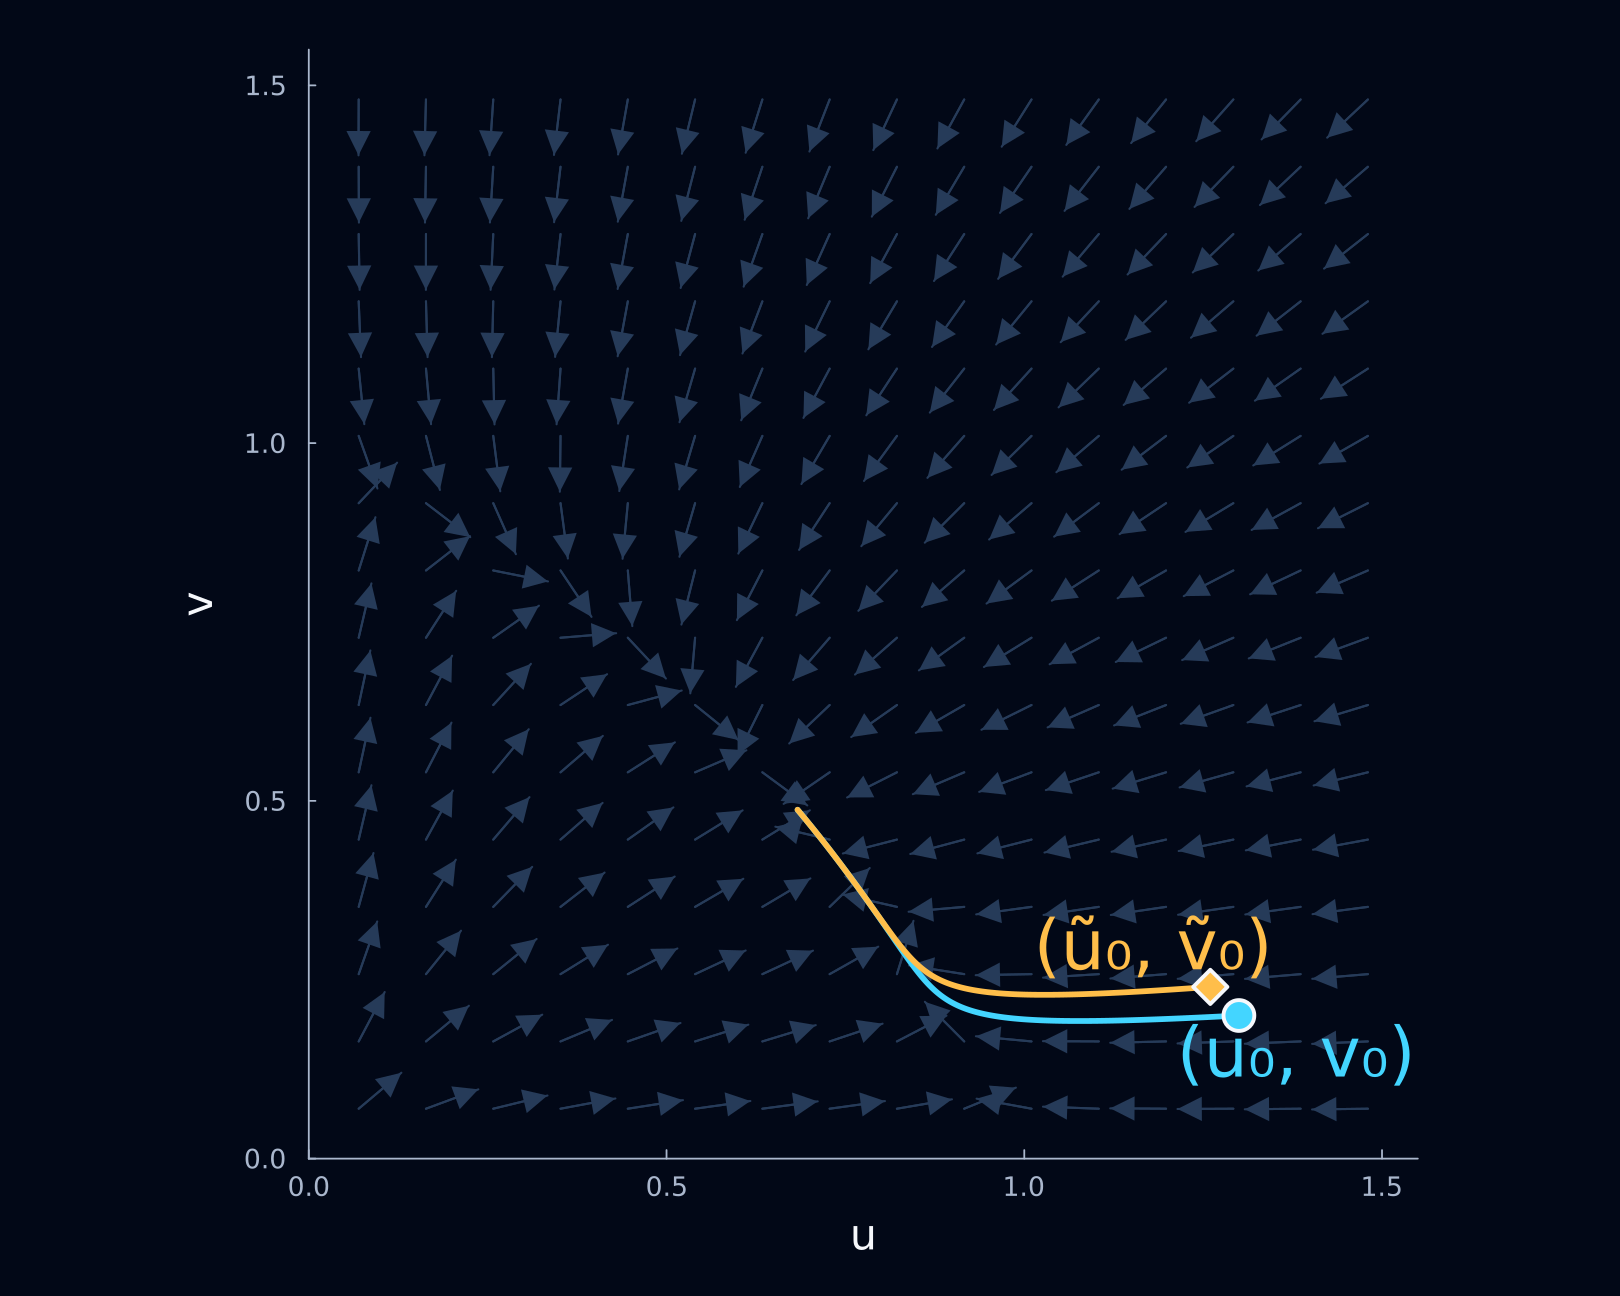
\includegraphics[
              width=\linewidth,
              height=3.80cm,
              keepaspectratio
            ]{figures/local_dynamics/stability_converging.png}

            \vspace{0.12cm}

            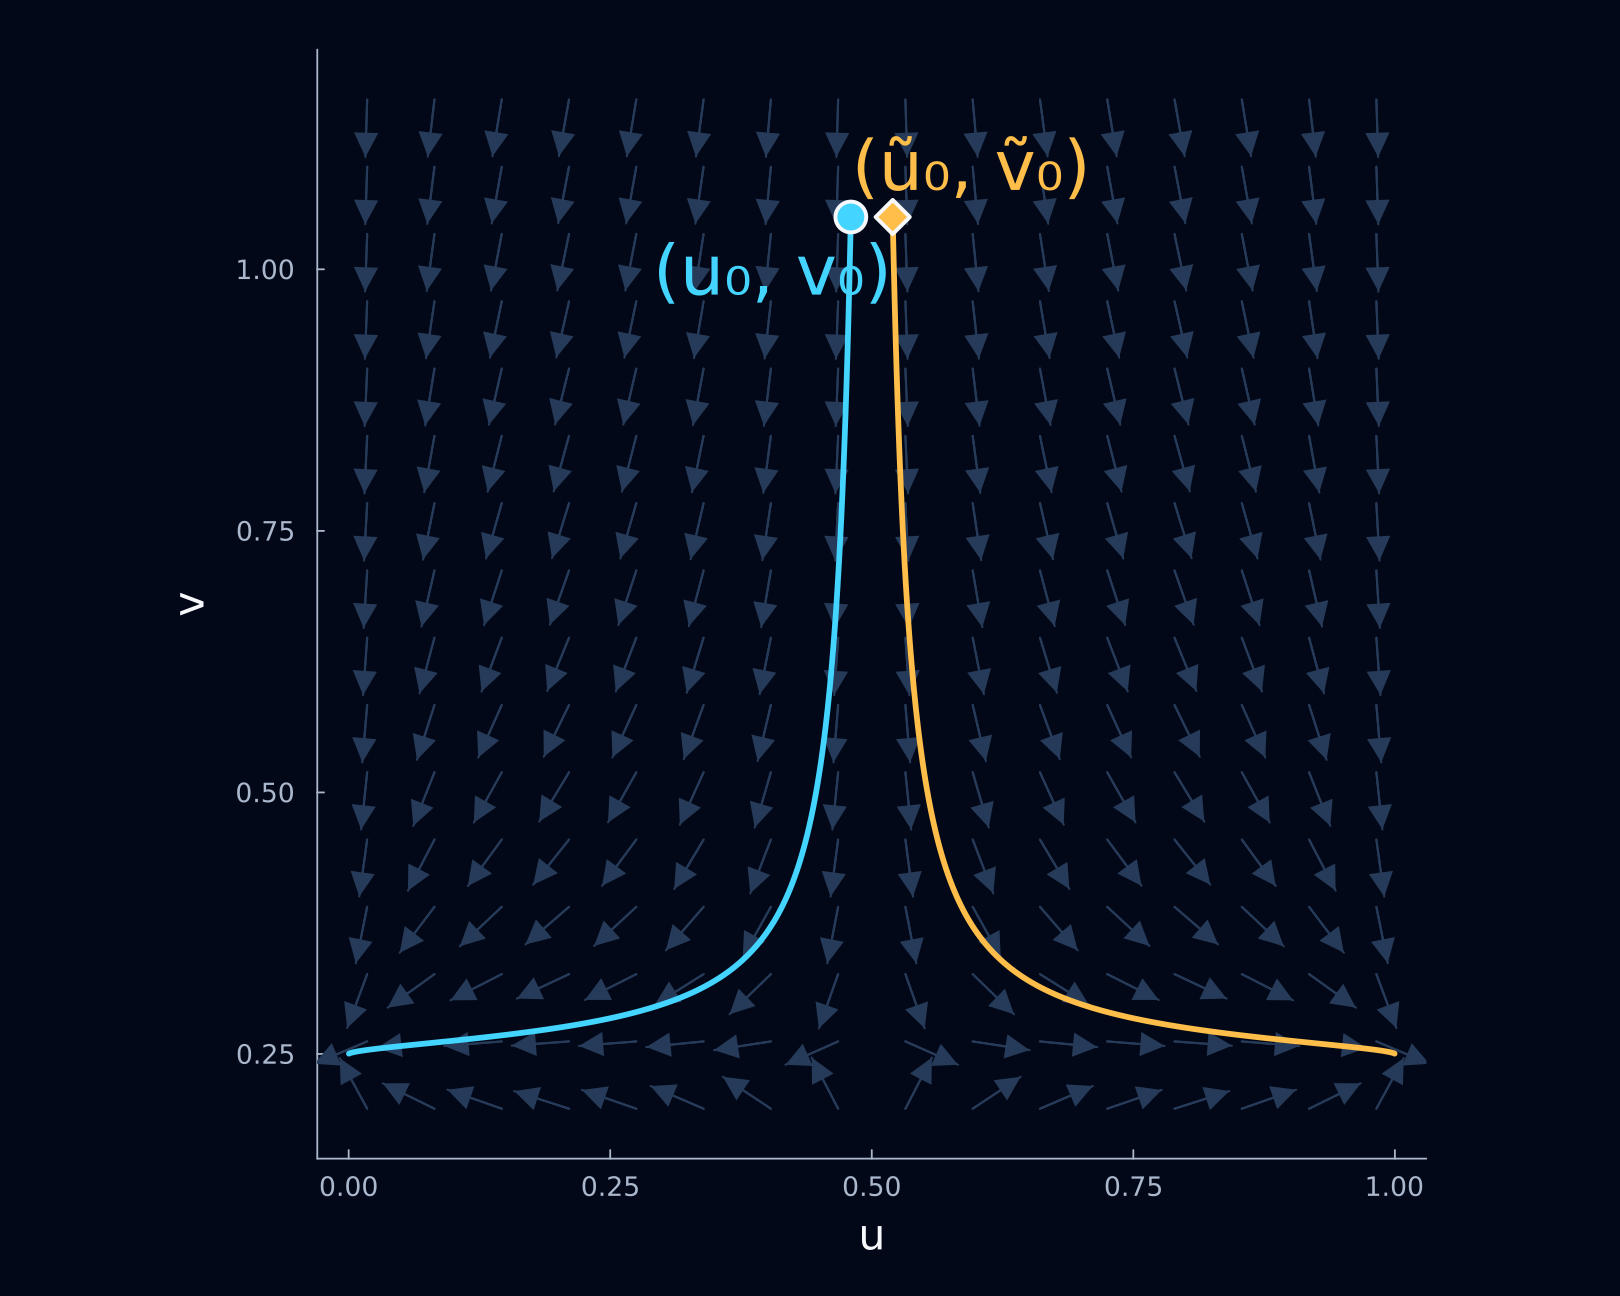
\includegraphics[
              width=\linewidth,
              height=3.80cm,
              keepaspectratio
            ]{figures/local_dynamics/stability_diverging.png}
          \end{column}

          \begin{column}{0.25\linewidth}

            \begin{minipage}[c][2.80cm][c]{\linewidth}
              {\color{HydraCyan}\bfseries
                \fontsize{7.7}{9.2}\selectfont
                STABLE
              \par}

              \vspace{0.08cm}

              {\color{HydraMuted}
                \fontsize{7.2}{9}\selectfont
                Nearby solutions converge
              \par}
            \end{minipage}

            \vspace{0.12cm}

            \begin{minipage}[c][2.80cm][c]{\linewidth}
              {\color{HydraGold}\bfseries
                \fontsize{7.7}{9.2}\selectfont
                UNSTABLE
              \par}

              \vspace{0.08cm}

              {\color{HydraMuted}
                \fontsize{7.2}{9}\selectfont
                Nearby solutions separate
              \par}
            \end{minipage}

          \end{column}

        \end{columns}


    \end{column}

  \end{columns}

\end{frame}

\begin{frame}{Stability of constant steady state}

\vspace{-0.75cm}

\begin{columns}[c,onlytextwidth]

  \begin{column}{0.45\textwidth}

      {\color{HydraWhite}\fontsize{11.4}{14.6}\selectfont
      \begin{align*}
        u(0)&=\bar u+\eta_0
        \\
        v(0)&=\bar v+\xi_0
      \end{align*}
      }

      \vspace{-0.52cm}

      {\color{HydraMuted}\fontsize{7.8}{9.6}\selectfont
        The perturbation is given by
      \par}

      \vspace{-0.68cm}

      {\color{HydraWhite}\fontsize{11.4}{14.6}\selectfont
      \begin{align*}
        \eta(t)&=u(t)-\bar u
        \\
        \xi(t)&=v(t)-\bar v
      \end{align*}
      }

      \vspace{-0.58cm}

      \HydraPoint[HydraCyan]
        {Asymptotically stable}
        {Every sufficiently small perturbation returns to the equilibrium.}

      \vspace{-0.46cm}

      {\color{HydraWhite}\fontsize{10.4}{13.2}\selectfont
      \begin{align*}
        \begin{aligned}
          \eta(t)&\longrightarrow0
          \\
          \xi(t)&\longrightarrow0
        \end{aligned}
        \qquad
        \text{as }t\longrightarrow\infty
      \end{align*}
      }

      \vspace{-0.36cm}

      \HydraPoint[HydraRed]
        {Unstable}
        {At least one arbitrarily small perturbation moves away.}

    \end{column}

  \begin{column}{0.51\textwidth}
    \centering

    % REPLACEABLE VISUAL
    % Replace the tikzpicture with:
    % \includegraphics[width=\linewidth,height=5.25cm,keepaspectratio]{figures/local_dynamics/...}
    \begin{tikzpicture}[x=0.93cm,y=0.93cm]
      \node[text=HydraCyan,font=\bfseries\fontsize{8}{9.5}\selectfont]
        at (1.75,5.15) {stable};
      \node[text=HydraRed,font=\bfseries\fontsize{8}{9.5}\selectfont]
        at (5.15,5.15) {unstable};

      \draw[HydraLine,line width=0.75pt]
        (3.43,0.55) -- (3.43,5.05);

      \fill[HydraWhite]
        (1.75,2.65) circle[radius=0.09cm];

      \draw[HydraCyan,line width=0.65pt,opacity=0.75]
        (1.75,2.65) circle[radius=0.42cm];

      \fill[HydraMuted]
      (0.65,4.10) circle[radius=0.055cm];

      \foreach \x/\y in {
        % 0.65/4.10,
        0.65/1.30,
        2.90/4.05,
        2.90/1.25
      }{
        \fill[HydraMuted]
          (\x,\y) circle[radius=0.055cm];

        \draw[-{Latex[length=2mm]},HydraCyan,line width=1.15pt]
          (\x,\y) -- ($(1.75,2.65)!0.68!(\x,\y)$);
      }

      \draw[-{Latex[length=2.1mm]},HydraCyan,line width=1.15pt]
        (0.72,3.92)
        .. controls (1.15,3.82) and (1.10,3.05)
        .. (1.55,2.83);

      \fill[HydraWhite]
        (5.15,2.65) circle[radius=0.09cm];

      \draw[HydraRed,line width=0.65pt,opacity=0.75]
        (5.15,2.65) circle[radius=0.42cm];

      \foreach \x/\y/\dx/\dy in {
        4.75/2.90/-0.90/0.72,
        4.82/2.30/-0.92/-0.78,
        5.50/2.95/0.85/0.82,
        5.52/2.30/0.82/-0.72
      }{
        \fill[HydraMuted]
          (\x,\y) circle[radius=0.055cm];

        \draw[-{Latex[length=2mm]},HydraRed,line width=1.15pt]
          (\x,\y) -- ++(\dx,\dy);
      }

      \node[
        anchor=north,
        text=HydraMuted,
        text width=2.8cm,
        align=center,
        font=\fontsize{7.1}{8.6}\selectfont
      ] at (1.75,0.38)
        {nearby states return};

      \node[
        anchor=north,
        text=HydraMuted,
        text width=2.8cm,
        align=center,
        font=\fontsize{7.1}{8.6}\selectfont
      ] at (5.15,0.38)
        {some nearby states escape};
    \end{tikzpicture}

  \end{column}

\end{columns}

\end{frame}


\begin{frame}{Linearized stability}

  \vspace{-0.22cm}

  {\color{HydraMuted}\fontsize{7.9}{9.6}\selectfont
    Near the steady state $(\bar u,\bar v)$ write
  \par}

  \vspace{-0.40cm}

  {\color{HydraWhite}\fontsize{10.2}{13}\selectfont
  \begin{align*}
    u=\bar u+\eta, \quad 
    v=\bar v+\xi
  \end{align*}
  }

  \vspace{-0.52cm}

  \begin{columns}[T,onlytextwidth]

    \begin{column}{0.62\textwidth}
      {\color{HydraGold}\bfseries\fontsize{7.7}{9.2}\selectfont
        TAYLOR EXPANSION\par}

      \vspace{-0.24cm}

      {\color{HydraWhite}\fontsize{8.6}{10.8}\selectfont
      \begin{align*}
        \partial_t \eta
        &=
        f(\bar u+\eta,\bar v+\xi)=f(\bar u,\bar v)
        +
        f_u(\bar u,\bar v)\eta
        +
        f_v(\bar u,\bar v)\xi
        +
        O\!\left(\lVert(\eta,\xi)\rVert^2\right) \\
        \partial_t \xi
        &=
        g(\bar u+\eta,\bar v+\xi)=g(\bar u,\bar v)
        +
        g_u(\bar u,\bar v)\eta
        +
        g_v(\bar u,\bar v)\xi
        +
        O\!\left(\lVert(\eta,\xi)\rVert^2\right)
      \end{align*}
      }

    \end{column}

    \begin{column}{0.34\textwidth}
      {\color{HydraGold}\bfseries\fontsize{7.7}{9.2}\selectfont
        \centering JACOBIAN\par}

      \vspace{-0.26cm}

    {\color{HydraWhite}\fontsize{10.2}{13}\selectfont
    \begin{align*}
      \boxed{
        J(\bar u,\bar v)
        =
        \begin{pmatrix}
          f_u(\bar u,\bar v) & f_v(\bar u,\bar v)
          \\
          g_u(\bar u,\bar v) & g_v(\bar u,\bar v)
        \end{pmatrix}
      }
    \end{align*}
    }


    \end{column}

  \end{columns}

  \vspace{-0.12cm}

  {\color{HydraGold}\bfseries\fontsize{7.7}{9.2}\selectfont
    NEGLECTING HIGHER-ORDER TERMS\par}

  \vspace{-0.32cm}

  {\color{HydraWhite}\bfseries\fontsize{12.8}{16}\selectfont
  \begin{align*}
    \boxed{
      \begin{pmatrix}
        \partial_t \eta
        \\
        \partial_t \xi
      \end{pmatrix}
      =
      J(\bar u,\bar v)
      \begin{pmatrix}
        \eta
        \\
        \xi
      \end{pmatrix}
    }
  \end{align*}
  }

  \vspace{-0.30cm}

  \HydraTakeaway{
    Close to the steady state, the Jacobian determines the leading-order dynamics
  }

\end{frame}


\begin{frame}{Eigenvalues of the Jacobian}

\vspace{-0.38cm}

\begin{columns}[c,onlytextwidth]

  \begin{column}{0.47\textwidth}
    \centering

    {\color{HydraGold}\bfseries\fontsize{8}{9.6}\selectfont
      LINEARIZED SYSTEM
    \par}

    \vspace{-0.20cm}

    {\color{HydraWhite}\fontsize{10.2}{13}\selectfont
    \begin{align*}
      \begin{pmatrix}
        \partial_t\eta
        \\
        \partial_t\xi
      \end{pmatrix}
      =
      J(\bar u,\bar v)
      \begin{pmatrix}
        \eta
        \\
        \xi
      \end{pmatrix}
    \end{align*}
    }
  \end{column}

  \begin{column}{0.49\textwidth}
    \centering

    % {\color{HydraGold}\bfseries\fontsize{8}{9.6}\selectfont
    %   JACOBIAN
    % \par}

    \vspace{-0.20cm}

    {\color{HydraWhite}\fontsize{9.2}{11.8}\selectfont
    \begin{align*}
      J(\bar u,\bar v)
      =
      \begin{pmatrix}
        f_u(\bar u,\bar v) & f_v(\bar u,\bar v)
        \\
        g_u(\bar u,\bar v) & g_v(\bar u,\bar v)
      \end{pmatrix}
    \end{align*}
    }

    \vspace{-0.34cm}

    {\color{HydraMuted}\fontsize{7.5}{9.2}\selectfont
      The eigenvalues are the roots of
    \par}

    \vspace{-0.28cm}

    {\color{HydraWhite}\fontsize{9.4}{12}\selectfont
    \begin{align*}
      \det\!\left(
        J(\bar u,\bar v)-\lambda I
      \right)=0
    \end{align*}
    }
  \end{column}

\end{columns}

\vspace{-0.32cm}

\begin{center}
  \begin{minipage}{0.90\textwidth}

    {\color{HydraGold}\bfseries\fontsize{9.2}{11}\selectfont
      THEOREM
    \par}

    \vspace{0.12cm}

    {\color{HydraWhite}\fontsize{8.4}{10.5}\selectfont
      Let $\lambda_1$ and $\lambda_2$ be the eigenvalues of
      $J(\bar u,\bar v)$
    \par}

    \vspace{0.18cm}

    {\color{HydraBody}\fontsize{8.6}{10.8}\selectfont
    \begin{itemize}
      \setlength{\itemsep}{0.28cm}

      \item
        If
        $\operatorname{Re}\lambda_1<0$
        and
        $\operatorname{Re}\lambda_2<0$
        then the steady state $(\bar u,\bar v)$ is
        \textcolor{HydraCyan}{\bfseries asymptotically stable}

      \item
        If
        $\operatorname{Re}\lambda_i>0$
        for at least one eigenvalue then the steady state
        $(\bar u,\bar v)$ is
        \textcolor{HydraRed}{\bfseries unstable}

    \end{itemize}
    }

    \vspace{0.12cm}

    {\color{HydraMuted}\fontsize{7.2}{8.8}\selectfont
      If an eigenvalue has zero real part, linearization alone may be inconclusive
    \par}

  \end{minipage}
\end{center}

\end{frame}


\begin{frame}{Eigenvalues}

\vspace{-0.48cm}

\begin{columns}[c,onlytextwidth]

  \begin{column}{0.43\textwidth}
    \centering

    \vspace{-0.24cm}

    {\color{HydraWhite}\fontsize{9.4}{12}\selectfont
    \begin{align*}
      \begin{pmatrix}
        \partial_t\eta
        \\
        \partial_t\xi
      \end{pmatrix}
      =
      J(\bar u,\bar v)
      \begin{pmatrix}
        \eta
        \\
        \xi
      \end{pmatrix}
    \end{align*}
    }
  \end{column}

  \begin{column}{0.53\textwidth}
    \centering


    \vspace{-0.24cm}

    {\color{HydraWhite}\fontsize{8.8}{11.2}\selectfont
    \begin{align*}
      J(\bar u,\bar v)
      =
      \begin{pmatrix}
        f_u(\bar u,\bar v) & f_v(\bar u,\bar v)
        \\
        g_u(\bar u,\bar v) & g_v(\bar u,\bar v)
      \end{pmatrix}
    \end{align*}
    }
  \end{column}

\end{columns}

\vspace{-0.38cm}

\begin{center}
  {\color{HydraGold}\bfseries\fontsize{7.8}{9.4}\selectfont
    CHARACTERISTIC EQUATION
  \par}

  \vspace{-0.24cm}

  {\color{HydraWhite}\fontsize{8.8}{11.2}\selectfont
  \begin{align*}
    \det\!\left(J-\lambda I\right)=
    \begin{vmatrix}
      f_u-\lambda & f_v
      \\
      g_u & g_v-\lambda
    \end{vmatrix}
    =
    (f_u-\lambda)(g_v-\lambda)-f_vg_u=
    \lambda^2-\operatorname{tr}(J)\lambda+\det(J)
  \end{align*}
  }
\end{center}
 
\vspace{-0.34cm}

\begin{columns}[t,onlytextwidth]

  \begin{column}{0.47\textwidth}

    {\color{HydraGold}\bfseries\fontsize{8.4}{10}\selectfont
      DETERMINANT
    \par}

    \vspace{0.10cm}

    {\color{HydraBody}\fontsize{7.8}{9.7}\selectfont
    \begin{itemize}
      \setlength{\itemsep}{0.20cm}

      \item
        If $\det(J)<0$, one eigenvalue is positive and one is negative

        \textcolor{HydraRed}{\bfseries The steady state is an unstable saddle}

      \item
        If $\det(J)>0$, real eigenvalues have the same sign or form a complex conjugate pair

        \textcolor{HydraMuted}{The trace determines the sign of their real parts}

    \end{itemize}
    }

  \end{column}

  \begin{column}{0.47\textwidth}

    {\color{HydraGold}\bfseries\fontsize{8.4}{10}\selectfont
      TRACE WHEN $\det(J)>0$
    \par}

    \vspace{0.10cm}

    {\color{HydraBody}\fontsize{7.8}{9.7}\selectfont
    \begin{itemize}
      \setlength{\itemsep}{0.20cm}

      \item
        If $\operatorname{tr}(J)<0$, both eigenvalues have negative real parts

        \textcolor{HydraCyan}{\bfseries The steady state is asymptotically stable}

      \item
        If $\operatorname{tr}(J)>0$, both eigenvalues have positive real parts

        \textcolor{HydraRed}{\bfseries The steady state is unstable}

    \end{itemize}
    }

  \end{column}

\end{columns}

\vspace{0.10cm}

\end{frame}

\begin{frame}{Eigenvalues determine local stability}

\vspace{-0.35cm}

\begin{center}
  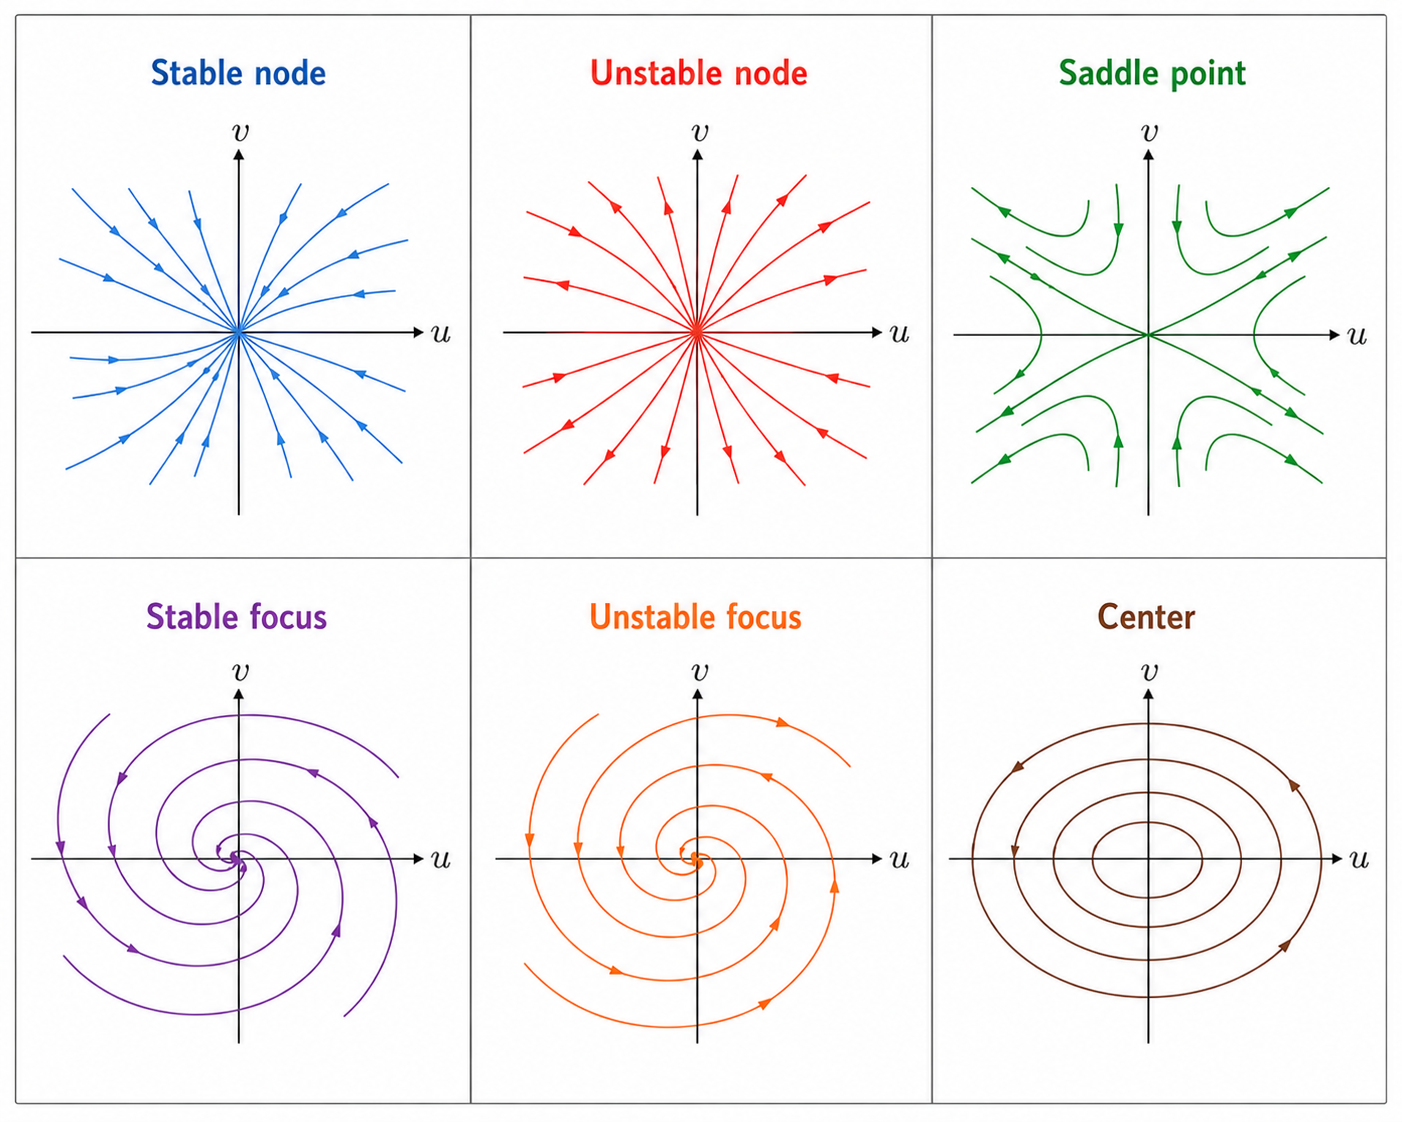
\includegraphics[
    width=0.98\textwidth,
    height=6.75cm,
    keepaspectratio
  ]{figures/local_dynamics/EigenvalueNode.png}
\end{center}

\end{frame}


\begin{frame}{Trace and determinant classify a two-variable equilibrium}

\vspace{-0.12cm}

\begin{columns}[c,onlytextwidth]

\begin{column}{0.46\textwidth}

  {\color{HydraWhite}\fontsize{9.6}{12.2}\selectfont
  \begin{align*}
    \det\!\left(
      J(\bar u,\bar v)-\lambda I
    \right)&=0
    \end{align*}
    \begin{align*}
    \boxed{
      \lambda^2
      -\operatorname{tr}(J)\lambda
      +\det(J)
      =0
    }
  \end{align*}
  }

  \vspace{-0.028cm}

  {\color{HydraMuted}\fontsize{7.8}{9.6}\selectfont
    Therefore
  \par}

  \vspace{-0.26cm}

  {\color{HydraWhite}\fontsize{9.6}{12.2}\selectfont
  \begin{align*}
    \lambda_1+\lambda_2
    &=
    \operatorname{tr}(J)
    \\
    \lambda_1\lambda_2
    &=
    \det(J)
  \end{align*}
  }



\end{column}

\begin{column}{0.50\textwidth}
  \centering

  % REPLACEABLE VISUAL
  % Replace the tikzpicture with:
  % \includegraphics[width=\linewidth,height=5.45cm,keepaspectratio]
  % {figures/local_dynamics/...}
  \begin{tikzpicture}[x=0.86cm,y=0.82cm]

    \fill[HydraRed,opacity=0.07]
      (0.35,0.48) rectangle (6.55,2.15);

    \fill[HydraCyan,opacity=0.07]
      (0.35,2.15) rectangle (3.45,5.55);

    \fill[HydraRed,opacity=0.05]
      (3.45,2.15) rectangle (6.55,5.55);

    \draw[-{Latex[length=2.3mm]},HydraMuted,line width=0.75pt]
      (0.35,2.15) -- (6.65,2.15)
      node[below,text=HydraMuted,
        font=\fontsize{7}{8.2}\selectfont]
      {$\operatorname{tr}J$};

    \draw[-{Latex[length=2.3mm]},HydraMuted,line width=0.75pt]
      (3.45,0.40) -- (3.45,5.65)
      node[left,text=HydraMuted,
        font=\fontsize{7}{8.2}\selectfont]
      {$\det J$};

    \draw[
      HydraGold,
      line width=1.25pt,
      domain=-2.55:2.55,
      samples=90
    ]
      plot ({3.45+\x},{2.15+0.47*\x*\x});

    \node[
      text=HydraMuted,
      font=\fontsize{6.8}{8.2}\selectfont
    ]
      at (1.30,1.25) {saddle};

    \node[
      text=HydraMuted,
      font=\fontsize{6.8}{8.2}\selectfont
    ]
      at (5.58,1.25) {saddle};

    \node[
      text=HydraCyan,
      font=\bfseries\fontsize{7.3}{8.8}\selectfont
    ]
      at (0.5,3.15) {stable node};

    \node[
      text=HydraCyan,
      font=\bfseries\fontsize{7.3}{8.8}\selectfont
    ]
      at (2.15,4.75) {stable spiral};

    \node[
      text=HydraRed,
      font=\bfseries\fontsize{7.3}{8.8}\selectfont
    ]
      at (6.25,3.15) {unstable node};

    \node[
      text=HydraRed,
      font=\bfseries\fontsize{7.3}{8.8}\selectfont
    ]
      at (4.65,4.75) {unstable spiral};

    \node[
      anchor=south east,
      text=HydraGold,
      font=\fontsize{6.9}{8.3}\selectfont
    ]
      at (6.38,5.30)
      {$\det J=\left(\operatorname{tr}J\right)^2/4$};

  \end{tikzpicture}

\end{column}

\end{columns}

\end{frame}




% \begin{frame}{Turing instability begins with a locally stable equilibrium}

%   \vspace{-0.05cm}

%   \begin{columns}[c,onlytextwidth]

%     \begin{column}{0.43\textwidth}
%       {\color{HydraGold}\bfseries\fontsize{7.8}{9.4}\selectfont
%         REACTIONS ALONE\par}

%       \vspace{-0.12cm}

%       {\color{HydraWhite}\fontsize{11.4}{14.4}\selectfont
%       \[
%         \dot{\boldsymbol\eta}=J_*\boldsymbol\eta
%       \]
%       }

%       \vspace{-0.22cm}

%       {\color{HydraWhite}\fontsize{10.8}{13.6}\selectfont
%       \[
%         \operatorname{tr}J_*<0
%         \qquad
%         \det J_*>0
%       \]
%       }

%       \vspace{-0.12cm}

%       \HydraPoint[HydraCyan]
%         {Homogeneous perturbations decay}
%         {If every point is perturbed in the same way, the local kinetics restore the equilibrium.}

%       \vspace{-0.24cm}

%       {\color{HydraMuted}\fontsize{7.8}{9.6}\selectfont
%         This stability is essential: the pattern must be created by spatial coupling, not by unstable reactions.
%       \par}
%     \end{column}

%     \begin{column}{0.53\textwidth}
%       {\color{HydraGold}\bfseries\fontsize{7.8}{9.4}\selectfont
%         ADD DIFFUSION\par}

%       \vspace{-0.14cm}

%       {\color{HydraWhite}\fontsize{11.4}{14.4}\selectfont
%       \[
%         \partial_t\boldsymbol\eta
%         =
%         J_*\boldsymbol\eta
%         +
%         \mathcal D\Delta\boldsymbol\eta
%       \]
%       }

%       \vspace{-0.24cm}

%       \centering

%       % REPLACEABLE VISUAL
%       % Replace the tikzpicture with:
%       % \includegraphics[width=\linewidth,height=2.75cm,keepaspectratio]{figures/local_dynamics/...}
%       \begin{tikzpicture}[x=0.96cm,y=0.96cm]
%         \draw[-{Latex[length=2.2mm]},HydraMuted,line width=0.75pt]
%           (0.35,0.55) -- (7.10,0.55)
%           node[below,text=HydraMuted,font=\fontsize{7}{8.2}\selectfont] {$x$};
%         \draw[HydraLine,line width=0.70pt] (0.45,2.10) -- (6.85,2.10);
%         \draw[HydraCyan,line width=1.55pt,domain=0.45:6.85,samples=100]
%           plot (\x,{2.10+0.55*cos(180*3*(\x-0.45)/6.40)});

%         \foreach \x in {0.55,1.25,...,6.85}{
%           \fill[HydraWhite,opacity=0.75] (\x,2.10) circle[radius=0.045cm];
%         }

%         \node[anchor=south west,text=HydraCyan,
%           font=\bfseries\fontsize{7.5}{9}\selectfont]
%           at (0.55,2.82) {nonconstant spatial perturbation};
%         \node[anchor=north,text=HydraMuted,text width=6.4cm,align=center,
%           font=\fontsize{7.1}{8.6}\selectfont]
%           at (3.65,0.16)
%           {different spatial modes will be tested separately};
%       \end{tikzpicture}

%       \vspace{-0.10cm}

%       {\color{HydraWhite}\bfseries\fontsize{9.6}{12}\selectfont
%         Can diffusion destabilize one nonconstant mode?
%       \par}
%     \end{column}

%   \end{columns}

%   \vspace{0.12cm}

%   \HydraTakeaway{
%     Turing instability is diffusion-driven loss of stability.
%   }

% \end{frame}
